\documentclass[a4paper, 12pt]{article}

\usepackage[T2A]{fontenc}
\usepackage[utf8]{inputenc}
\usepackage[english, russian]{babel}
\usepackage{amsfonts}
\usepackage{amsmath}
\usepackage{multirow}
\usepackage{multicol}
\usepackage{tabularx}
\usepackage{hhline}
\usepackage{titlesec}

\usepackage{graphicx}
\graphicspath{{}}
\DeclareGraphicsExtensions{.pdf,.png,.jpg}

\newcommand{\sectionbreak}{\clearpage}

\usepackage{xltxtra}
\usepackage[main=russian,english]{babel}


\begin{document}
    \title{Доклад про AVL-дерево}
    \author{Еремеев Тимур}
    \date{10 апреля 2022}

    \maketitle

    \tableofcontents

    \section*{Введение}
    AVL"=дерево "--- сбалансированное по высоте бинарное дерево поиска: для каждой его вершины высота её двух поддеревьев различается не более чем на 1.

AVL "--- аббревиатура, образованная первыми буквами создателей (советских учёных) Г. М. Адельсон-Вельского и Е. М. Ландиса.

    \section*{Общие свойства}
    В AVL"=дереве высоты $h$ имеется не меньше $F_h$ узлов, где $F_h$ "--- число Фибоначчи.
Поскольку $F_n = \frac{(\frac{1 + \sqrt{5}}{2})^n - (\frac{1 - \sqrt{5}}{2})^n}{\sqrt{5}} =
\frac{\phi^n - (-\phi)^{-n}}{\phi - (-\phi)^{-1}}$,
где $\frac{\phi^n - (-\phi)^{-n}}{\phi - (-\phi)^{-1}}$ "--- золотое сечение,
то имеем оценку высоты AVL-дерева $h = Q(\lg(n))$,
где $n$ "--- число узлов. Следует помнить, что $Q(\lg(n))$ "--- мажоранта,
и её можно использовать только для оценки
(Например, если в дереве только два узла, значит в дереве два уровня,
хотя $\lg(2) = 1$. Для точной оценки глубины дерева следует использовать пользовательскую программу.

% листинг
\begin{}
function TreeDepth(Tree : TAVLTree) : byte;
begin
   if Tree <> nil then
      result := 1 + Max(TreeDepth(Tree^.left),TreeDepth(Tree^.right))
  else
      result := 0;
end;
\end{}

Тип Дерева можно описать так:

% ещё один листинг
\begin{}
TKey = LongInt;
TInfo = LongInt;
TBalance = -1..1;
TAVLTree = ^ TAVLNode;
  TAVLNode = record
    left, right : TAVLTree;
    key : TKey;
    info : TInfo;
{ Поле определяющее сбалансированность вершины }
    balance : TBalance;
  end;
\end{}

    \section*{Балансировка}
    Относительно AVL"=дерева балансировкой вершины называется операция,
которая в случае разницы высот левого и правого поддеревьев $= 2$,
изменяет связи предок-потомок в поддереве данной вершины так,
что разница становится $ \leqslant 1$, иначе ничего не меняет.
Указанный результат получается вращениями поддерева данной вершины.

Используется 4 типа вращений:

\subsection*{Малое левое вращение}

%картинка 1
\begin{figure}[ht]
    \includegraphics[width = \textwidth]{1.gif}
    
    \caption{Схематическое изображение малого левого вращения}    
\end{figure}

Данное вращение используется тогда,
когда (высота $b$"=поддерева; $L$ "--- высота )
$= 2$ и высота $С \leqslant$ высота $R$.

\subsection*{Большое левое вращение}

%картинка 2
\begin{figure}[ht]
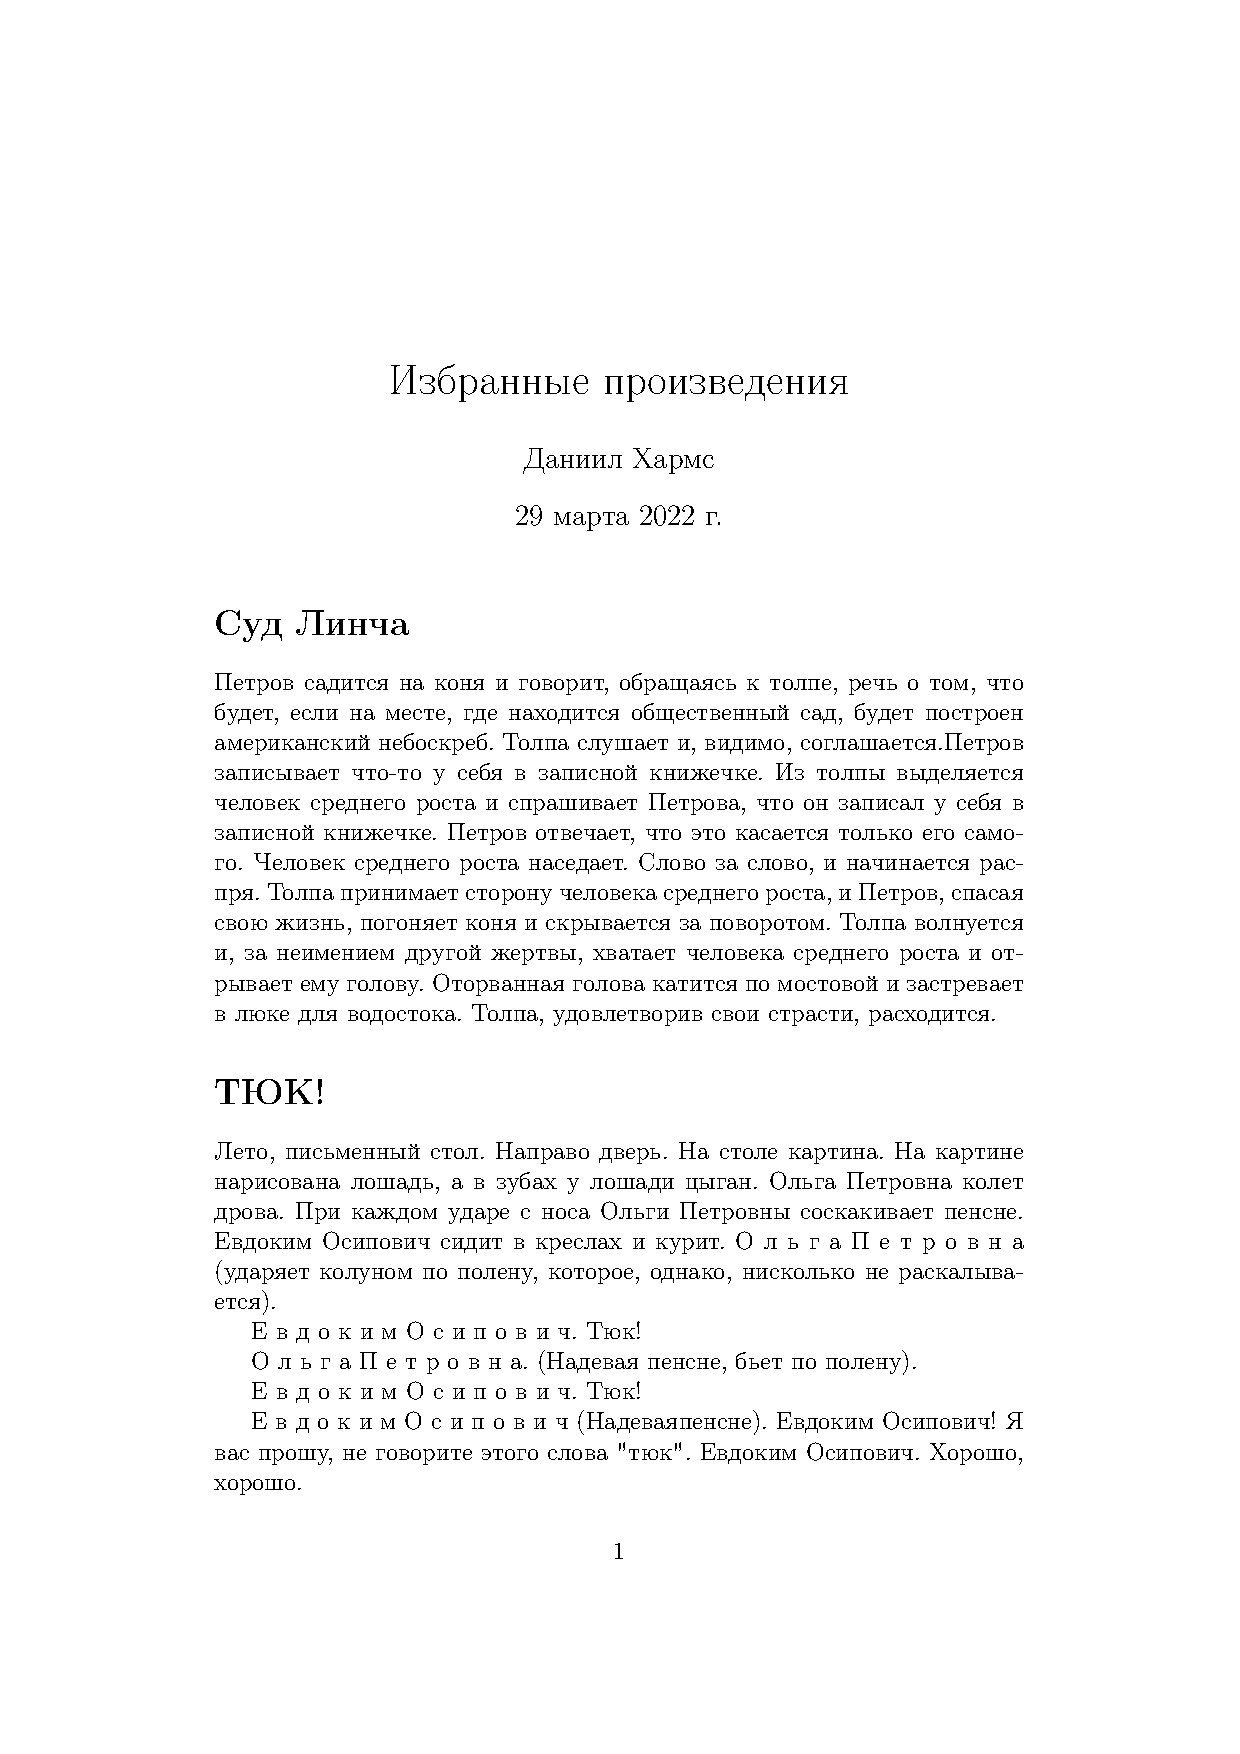
\includegraphics[width = \textwidth]{2.gif}

\caption{Схематическое изображение большого левого вращения}
\end{figure}

Данное вращение используется тогда,
когда (высота $b$"=поддерева; $L$ "--- высота)
$= 2$ и высота $c$"=поддерева $>$ высота $R$.

\subsection*{Малое правое вращение}

%картинка 3
\begin{figure}[ht]
    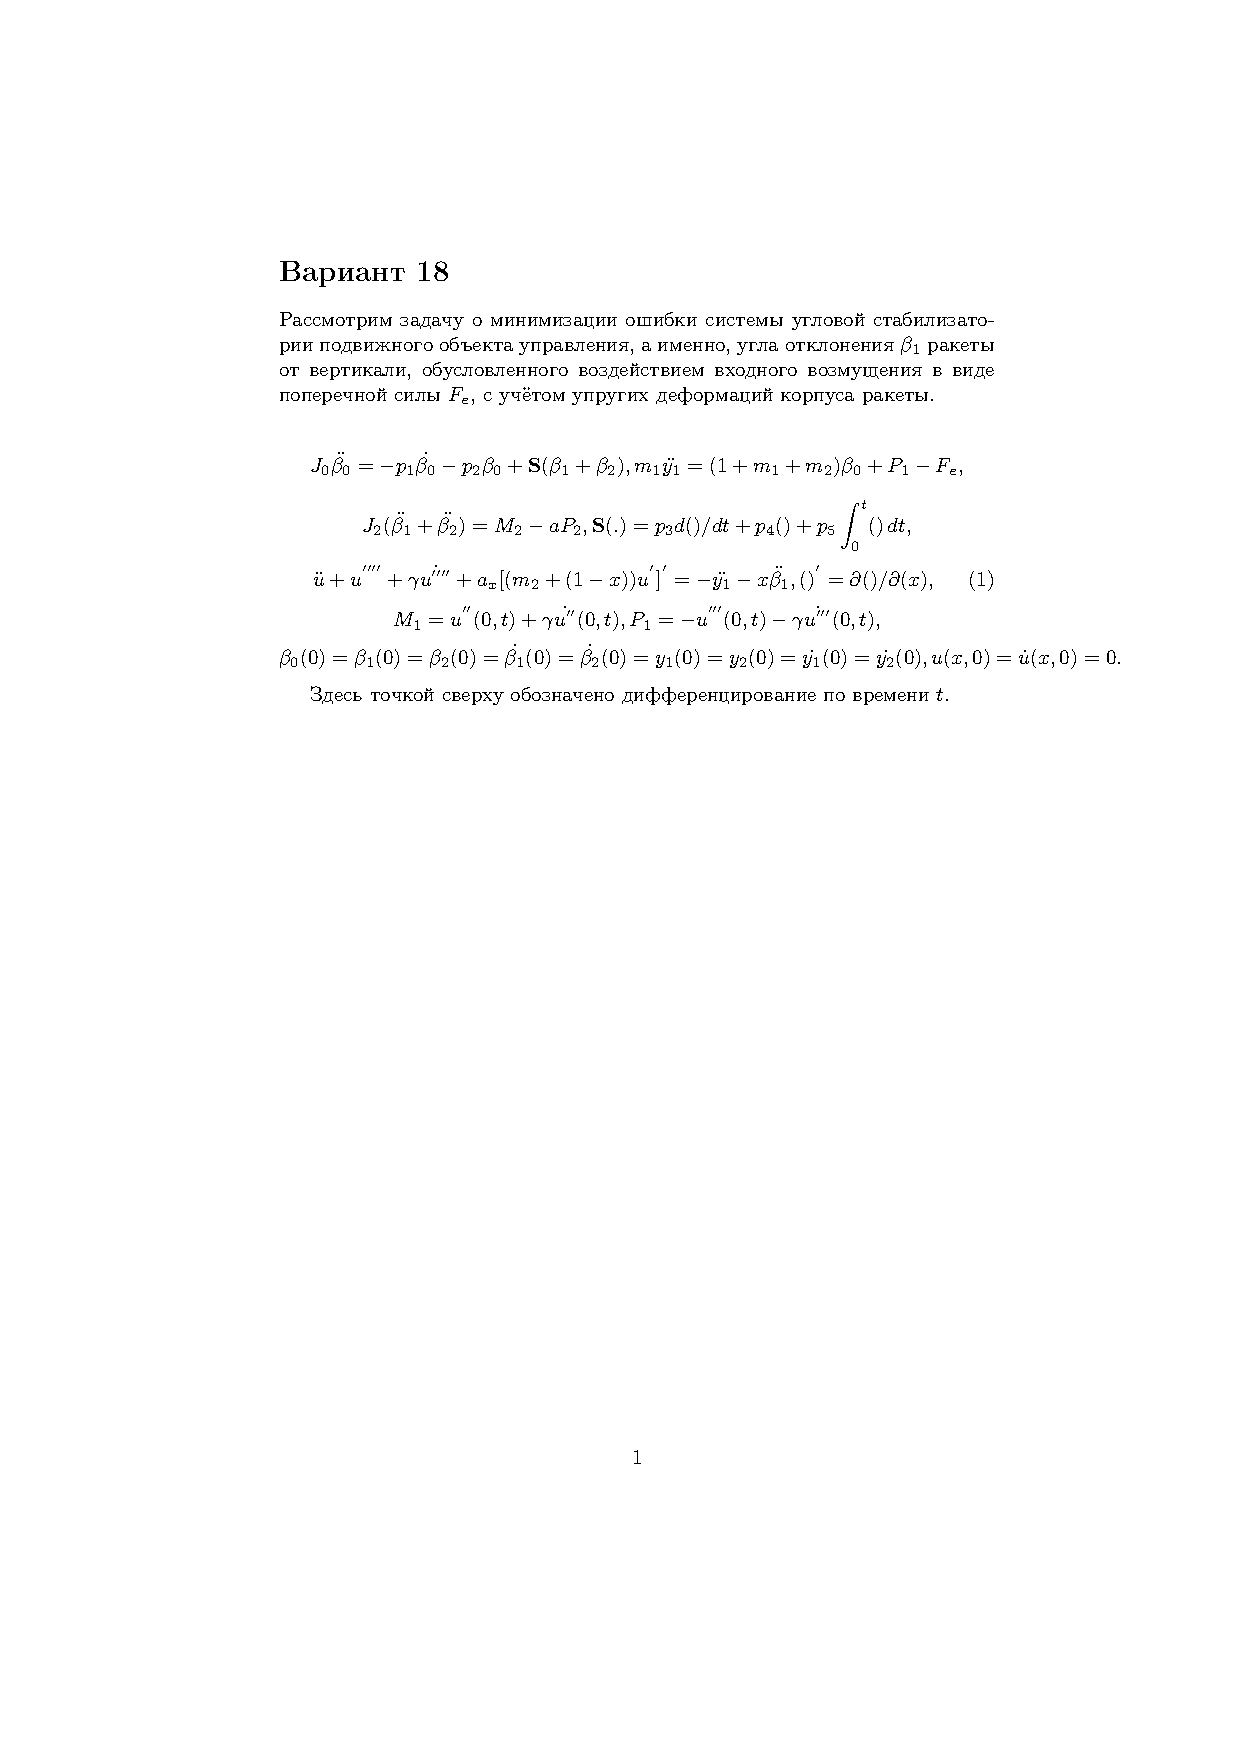
\includegraphics[width = \textwidth]{3.gif}
    
    \caption{Схематическое изображение малого правого вращения}
\end{figure}

Данное вращение используется тогда,
когда (высота $b$"=поддерева "--- высота $R$)
$= 2$ и высота $С \leqslant $ высоты $L$.

\subsection*{Большое правое вращение}

%картинка 4
\begin{figure}[ht]
    \includegraphics[width = \textwidth]{4.gif}
    
    \caption{Схематическое изображение большого правого вращения}

\end{figure}

Данное вращение используется тогда, когда (высота $b$"=поддерева; $R$ "--- высота)
$= 2$ ивысота $c$"=поддерева $ > $ высота $L$.
В каждом случае достаточно просто доказать то, 
что операция приводит к нужному результату и
что полная высота уменьшается не более чем на $1$ и не может увеличиться.
Из-за условия сбалансированности высота дерева $O(\lg(N))$,
где $N$ "--- количество вершин, поэтому добавление элемента требует $Q(\lg(N))$ операций.

    \section*{Алгоритм добавления вершин}
    Показатель сбалансированности в дальнейшем будем интерпретировать
как разность между высотой левого и правого поддерева,
а алгоритм будет основаться на типе TAVLTree, описанном выше.
Непосредственно при вставке (листу) присваивается нулевой баланс.
Процесс включения вершины состоит из трех частей:

\begin{enumerate}
    \item Прохода по пути поиска, пока не убедимся, что ключа в дереве нет.
    \item Включения новой вершины в дерево и определения результирующих показателей балансировки.
    \item "Отступления" назад по пути поиска и проверки в каждой вершине показателя сбалансированности.
    Если необходимо - балансировка
\end{enumerate}

Расширим список параметров обычной процедуры вставки параметром-переменной flag,
означающим, что высота дерева увеличилась.
Предположим, что процесс из левой ветви возвращается к родителю (рекурсия идет назад),
тогда возможны три случая:
{$h_1$ "--- высота левого поддерева, $h_r$- высота правого поддерева}
Включение вершины в левое поддерево приведет к

\begin{enumerate}
    \item $ $: выровняется $ $. Ничего делать не нужно.
    \item $ $: теперь левое поддерево будет больше на единицу,
    но балансировка пока не требуется.
    \item $ $: теперь $ $ "--- $ $, - требуется балансировка.
\end{enumerate}

В третьей ситуации требуется определить балансировку левого поддерева.
Если левое поддерево этой вершины ($Tree^.left^.left$) выше правого ($Tree^.left^.right$),
то требуется большое правое вращение, иначе хватит малого правого.
Аналогичные (симметричные) рассуждения можно привести и для включение в правое поддерево.
Процедура вставки, предложенная Н.Виртом

%листинг
\begin{}
procedure TAVL.InsertNode(Var Tree : TAVLTree; const akey : TKey; const ainfo : TInfo; Var flag : Boolean);
 Var
 Node1, Node2 : TAVLTree;
 begin
 if Tree = nil then
  begin
    New(Tree);
    flag := true;
    with Tree^ do
      begin
        key := akey;
        info := ainfo;
        left := nil;
        right := nil;
        balance := 0;
      end;
    inc(AVL.FNodes);
  end
 else if Tree^.key > akey then
  begin
    InsertNode(Tree^.left,akey,ainfo,flag);
    if flag then
      case Tree^.balance of
      1 : begin Tree^.balance := 0; flag := false; end;
      0 : Tree^.balance := -1;
      -1 :   { Balance }
        begin
         Node1 := Tree^.left;
         if Node1^.balance = -1 then
          { LL }
            begin
              Tree^.left := Node1^.right;
              Node1^.right := Tree;
              Tree^.balance := 0;
              Tree := Node1;
            end
         else
            {LR}
            begin
              Node2 := Node1^.right;
              Node1^.right :=  Node2^.left;
              Node2^.left := Node1;
              Tree^.left := Node2^.right;
              Node2^.right := Tree;
              if Node2^.balance = -1 then Tree^.balance := 1 else Tree^.balance := 0;
              if Node2^.balance = 1 then Node1^.balance := -1 else Node1^.balance := 0;
              Tree := Node2;
            end;
         Tree^.balance := 0;
         flag := false
        end
      end
  end
 else if Tree^.key < akey then
  begin
    InsertNode(Tree^.right,akey,ainfo,flag);
    if flag then
      case Tree^.balance of
      -1 : begin Tree^.balance := 0; flag := false; end;
      0 : Tree^.balance := 1;
      1 :   { Balance }
        begin
         Node1 := Tree^.right;
         if Node1^.balance = 1 then
          { RR }
            begin
              Tree^.right := Node1^.left;
              Node1^.left := Tree;
              Tree^.balance := 0;
              Tree := Node1;
            end
         else
            {RL}
            begin
              Node2 := Node1^.left;
              Node1^.left :=  Node2^.right;
              Node2^.right := Node1;
              Tree^.right := Node2^.left;
              Node2^.left := Tree;
              if Node2^.balance = 1 then Tree^.balance := -1 else Tree^.balance := 0;
              if Node2^.balance = -1 then Node1^.balance := 1 else Node1^.balance := 0;
              Tree := Node2;
            end;
         Tree^.balance := 0;
         flag := false
        end
      end
  end
 end;
\end{}

    \section*{Алгоритм удаления вершин}
    Для простоты опишем рекурсивный алгоритм удаления.
Если вершина "--- лист, то удалим её и вызовем балансировку всех её предков в порядке от родителя к корню.
Иначе найдём самую близкую по значению вершину в поддереве наибольшей высоты (правом или левом) и переместим её на место удаляемой вершины,
при этом вызвав процедуру её удаления.

Докажем, что данный алгоритм сохраняет балансировку.
Для этого докажем по индукции по высоте дерева,
что после удаления некоторой вершины из дерева и
последующей балансировки высота дерева уменьшается не более, чем на 1.
База индукции: Для листа очевидно верно.
Шаг индукции: Либо условие балансированности в корне (после удаления корень может изменится) не нарушилось,
тогда высота данного дерева не изменилась,
либо уменьшилось строго меньшее из поддеревьев $ $
высота до балансировки не изменилась $ $
после уменьшится не более чем на 1.

Очевидно, в результате указанных действий процедура удаления вызывается не более 3 раз,
так как у вершины, удаляемой по 2-му вызову, нет одного из поддеревьев.
Но поиск ближайшего каждый раз требует $O(N)$ операций,
отсюда видна очевидная оптимизация:
поиск ближайшей вершины производится по краю поддерева.
Отсюда количество действий $O(\lg(N))$.

    \section*{Расстановка балансов при удалении}
    Как уже говорилось, если удаляемая вершина"="лист, то она удаляется,
и обратный обход дерева происходит от родителя удалённого листа.
Если не лист "--- ей находится «замена», и обратный обход дерева происходит от родителя «замены».
Непосредственно после удаления элемента "--- «замена» получает баланс удаляемого узла.

При обратном обходе: если при переходе к родителю пришли слева "--- баланс увеличивается на $1$,
если же пришли справа "--- уменьшается на $1$.

Это делается до тех пор, пока при изменении баланса он не станет равным $-1$ или $1$
(обратите внимание на различие с вставкой элемента!):
в данном случае такое изменение баланса будет гласить о неизменной дельта-высоте поддеревьев.
Повороты происходят по тем же правилам, что и при вставке.

    \section*{Расстановка при одинарном повороте}
    Обозначим:

«Current» "--- узел, баланс которого равен $-2$ или $2$:
то есть тот, который нужно повернуть (на схеме - элемент a)

«Pivot» "--- ось вращения. $+2$: левый сын Current'а, $-2$: правый сын Current'а (на схеме "--- элемент $b$)

Если поворот осуществляется при вставке элемента, то баланс Pivot'а равен либо $1$, либо $-1$.
В таком случае после поворота балансы обоих устанавливаются равными $0$.

При удалении всё иначе: баланс Pivot'а может стать равным $0$ (в этом легко убедиться).

Приведём сводную таблицу зависимости финальных балансов от направления поворота и исходного баланса узла Pivot:

\begin{table*}
    \begin{tabular}{|c|c|c|c|c|c|}
                                 & Type IIB         & Type IIA            & E8 x E8 Гетеротическая & SO(32) Гетеротическая & Type I               \\
        \hline
        Тип струны               & Замкнутые        & Замкнутые           & Замкнутые              & Замкнутые             & Открытые и замкнутые \\
        \hline
        10d Суперсимметрия       &$N=2$ (киральная) & $N=2$ (некиральная) & $N = 1$                & $N = 1$               & $N = 1$              \\
        \hline
        10d Калибровочные группы & нет              & нет                 & E8 x E8                & SQ(32)                & SQ(32)               \\
        \hline
        D"=браны                 & -1, 1, 3, 5, 7   & 0, 2, 4, 6, 8       & нет                    & нет                   & 1, 5, 9              \\ 
        \hline
    \end{tabular}
\end{table*}

    \section*{Расстановка балансов при двойном повороте}
    Pivot и Current "--- те же самые, но добавляется третий участник поворота.
Обозначим его за «Bottom»: это (при двойном правом повороте) левый сын Pivot'а,
а при двойном левом "--- правый сын Pivot'а.

При данном повороте "--- Bottom в результате всегда приобретает баланс $0$,
но от его исходного баланса зависит расстановка балансов для Pivot и Current.

Приведём сводную таблицу зависимости финальных балансов от направления поворота и исходного баланса узла Bottom:

\begin{table*}
    \begin{tabular}{|c|c|c|c|c|c|}
                                 & Type IIB         & Type IIA            & E8 x E8 Гетеротическая & SO(32) Гетеротическая & Type I               \\
        \hline
        Тип струны               & Замкнутые        & Замкнутые           & Замкнутые              & Замкнутые             & Открытые и замкнутые \\
        \hline
        10d Суперсимметрия       &$N=2$ (киральная) & $N=2$ (некиральная) & $N = 1$                & $N = 1$               & $N = 1$              \\
        \hline
        10d Калибровочные группы & нет              & нет                 & E8 x E8                & SQ(32)                & SQ(32)               \\
        \hline
        D"=браны                 & -1, 1, 3, 5, 7   & 0, 2, 4, 6, 8       & нет                    & нет                   & 1, 5, 9              \\ 
        \hline
    \end{tabular}
\end{table*}

    \section*{Оценка эффективности}
    Г.М.Адельсон-Вельский и Е.М.Ландис доказали теорему,
согласно которой высота AVL"=дерева с $N$ внутренними вершинами заключена между $log2(N+1)$ и $1.4404*log2(N+2)-0.328$,
то есть высота AVL"=дерева никогда не превысит высоту идеально сбалансированного дерева более,чем на $45\%$.
Для больших N имеет место оценка $1.04*log2(N)$.
Таким образом, выполнение основных операций $1"=3$ требует порядка $log2(N)$ сравнений.
Экспериментально выяснено, что одна балансировка приходится на каждые два включения и на каждые пять исключений.

    \section*{Список используемой литературы}
    \begin{enumerate}
    \item Вирт Н. Алгоритмы и структуры данных М.:Мир, 1989. Глава 4.5 (С. 272-286)
    \item Г. М. Адельсон"=Вельский, Е. М. Ландис. Один алгоритм организации информации // Доклады АН СССР. 1962. Т.146, № 2. C. 263–266.
\end{enumerate}

\end{document}